\documentclass[UTF8,a4paper,zihao=-4,fontset=none]{ctexart}
\usepackage[margin=24mm]{geometry}
\usepackage{amsmath,booktabs,graphicx,tabularx,float,longtable,array}
\usepackage[unicode,hidelinks,hypertexnames=false]{hyperref}
\usepackage{url}
\usepackage{xcolor}
\usepackage{fontspec}
\setmainfont[Path=fonts/,AutoFakeBold=2,
 ItalicFont=NotoSerif-Regular.ttf,SlantedFont=NotoSerif-Regular.ttf]{NotoSerif-Regular.ttf}
\setsansfont[Path=fonts/,BoldFont=SourceHanSansCN-Bold.ttf]{SourceHanSansCN-Regular.ttf}
\setmonofont[Path=fonts/]{NotoSans-Regular.ttf}
\setCJKmainfont[
  Path=fonts/,
  ItalicFont=SourceHanSansCN-Regular.ttf,
  BoldFont=SourceHanSansCN-Bold.ttf
]{SourceHanSansCN-Regular.ttf}
\setCJKsansfont[
  Path=fonts/,
  ItalicFont=SourceHanSansCN-Regular.ttf,
  BoldFont=SourceHanSansCN-Bold.ttf
]{SourceHanSansCN-Regular.ttf}
\setCJKmonofont[Path=fonts/]{SourceHanSansCN-Regular.ttf}
\makeatletter
\g@addto@macro\UrlBreaks{\do\_\do\-}
\makeatother
\setlength{\parskip}{0.28em}
\linespread{1}
\renewcommand{\normalsize}{\fontsize{14pt}{25pt}\selectfont}
\setcounter{tocdepth}{1}
\newcommand{\km}{\ensuremath{\mathrm{km}^2}}
\newcommand{\code}[1]{\nolinkurl{#1}}
\newcommand{\todo}[1]{\textbf{[待人工核对：#1]}}
\setlength{\emergencystretch}{2em}

\begin{document}

\begin{titlepage}
\centering
\vspace*{24mm}
{\zihao{3} AI for Science 课程大作业\par}
\vspace{18mm}
{\sffamily\bfseries\zihao{1} 面向洪涝空间暴露分析的\\[4mm] AI 智能体实践探索\par}
\vspace{9mm}
{\zihao{3} FloodLab：遥感评估、QGIS 工具调用与交互制图\par}
\vfill
\begin{tabular}{rl}
团队成员：& 史森、王申杰、尹胜、李广鹏、刘士涵\\[3mm]
研究方向：& 计算机视觉、具身智能、智能体、遥感与物理仿真\\[3mm]
报告日期：& 2026 年 11 月 21 日
\end{tabular}
\vspace{18mm}
\end{titlepage}

\tableofcontents
\clearpage

\begin{abstract}
用户问“哪里发生了洪涝”，并不等于已经选定了研究区、观测日期和可计算的图层。本文实现本地应用 FloodLab 0.6.0：Pi 智能体检索事件，区分新闻线索与可下载的观测产品；用户确定问题后，QGIS 执行空间计算，输入、来源和地图写入该对话的工作区。瓦伦西亚案例检验需求变化：改变道路类别和网格尺度后，156、42、624 个网格的道路长度及暴露率均通过独立程序逐格核验。克里特岛案例检验数据未预装时的执行能力：智能体找到 Kastelli 的观测产品，下载 88 个多边形，合并后积水及洪水痕迹面积为 0.2413 \km。两项验证分别回答“修改口径后能否算对”和“能否为另一个事件找到数据并完成制图”。上游遥感实验另在 Sen1Floods11 官方测试清单评估阈值法与预训练网络，不把像元分类精度当作智能体评价。现有结果支持上述案例的可执行性，尚不能估计任意地点的检索召回率或开放任务成功率。

\noindent\textbf{关键词：} AI for Science；洪涝遥感；Sentinel-1；变化检测；AI Agent；QGIS；证据门控
\end{abstract}

\section{引言}
\subsection{为什么需要事件级制图}
在一个普通的图像分类任务中，输入和标签通常已经由实验者固定，模型输出一个类别或一张掩膜即可评价。但洪涝遥感制图是一个带有时间、空间和证据关系的科学工作流。用户说“把洪水画出来”时，至少可能有四种含义：画当前观测到的低散射水面、画灾前后新增的水面、复核已有官方产品，或者制作一张能够用于汇报和后续编辑的专题地图。如果没有先说明这些含义，算法即使能够输出一张漂亮的图，也可能回答了错误的问题。

本项目把目标拆成三个可以分别检查的问题。第一，在具有人工水体标注的官方测试清单上，预训练监督模型相对于 VH 阈值法总体改善多少，在哪里反而变差？第二，真实事件中，多时相变化候选与外部参考之间有哪些重叠和分歧，怎样在地图中表达？第三，也是产品的核心问题：当用户改变道路类别、网格尺度和排名指标时，语言模型能否实际重新组织空间操作，更新统计与地图，同时保留可核查的来历？

\subsection{相关工作与选题定位}
GIS Copilot 已研究把语言模型与 QGIS 工具及文档结合，使自然语言请求转为多步空间分析流程\cite{giscopilot}。因此，“大模型调用 QGIS”本身不是本项目提出的新方向。CartoAgent 进一步研究多模态模型参与地图风格迁移和评价\cite{cartoagent}；其任务范围与本项目的道路暴露计算不同，不能把制图外观改善等同于空间分析正确。本项目借鉴工具调用和视觉反馈思路，选择一个能在本机运行、能逐格复核、也能直接展示给使用者的课程级问题。

具体选择不是研发新的洪水分割网络，也不是把通用编程助手已有能力重新命名。FloodLab 的交付价值在于将固定研究区的数据、可执行 GIS 工具、连续任务状态、数值复核和制图成果组织为一个可操作应用。对于参数完全固定的一次分析，人工脚本更简单；需要考察 Agent 的情形是用户逐轮改变要求，而系统必须理解变化会影响哪些步骤。是否比通用 Agent 更可靠仍需公平实验，本项目不预设答案，也未实测与 Codex 的优劣。

\subsection{项目边界}
本文报告的是科研型分析产品，不是应急业务系统，也不是测绘成果鉴定。雷达变化候选不自动等于洪水边界；低后向散射还可能来自阴影、湿土、农田、粗糙度变化或观测几何差异。EMS 产品在本项目中仅作为时间不完全同步的外部参考，用于研究“来源之间的重叠和分歧”，不能被称为同期真值。数据中没有水深观测、体积反演和损失统计，因此 Agent 对这类请求必须拒绝，而不是从二维掩膜推导不存在的物理量。

项目交付桌面工作台、研究代码、栅格与矢量成果、可编辑 QGIS 工程及本报告。Horta Sud 的道路暴露实验使用预装 EMS 轮廓；跨事件工作流则可以下载 Copernicus EMS 已发布的观测多边形。二者的数据范围不同：外地若只有新闻而没有匹配的观测范围，系统可以整理简报，但不能借用瓦伦西亚图层计算当地受淹面积。

\section{任务设计与实施方法}
\subsection{官方测试集与预训练权重}
单期实验使用 Sen1Floods11 v1.1 人工标注部分及官方 \code{flood_test_data.csv} 清单\cite{sen1,senrepo}。清单配对 $512\times512$ 像元 Sentinel-1 双极化后向散射与人工水体图层；以浮点 dB 值读取 VV、VH，标签 $1$ 为水、$0$ 为非水、$-1$ 不作参考。两种方法读入完全相同的影像。预测在读取参考标签前完成，未使用测试标注拟合阈值、重新训练网络或挑选权重。清单包含十个按事件命名的分组，不能据此推断十个事件均与训练区隔离。

网络采用公开存储中的人工标注训练检查点，其完整对象名见输入清单。代码在加载前检查固定 SHA-256，并严格校验参数名与形状。清单 \code{outputs/inputs-test.json} 记录 182 项输入（90 对影像与标注、一份官方测试清单、一份检查点）的路径、字节数和散列。本机权重文件的字节数和 MD5 均与公开对象元数据一致；测试清单的 SHA-256 与公开存储的新下载副本一致。这些检查不代表另行复核了原作者的训练数据。

\subsection{事件与研究区}
研究对象为西班牙瓦伦西亚附近 2024 年 10 月下旬洪涝事件\cite{ems}。下载窗口为经纬度框 $[-0.645,39.230,-0.269,39.505]$，投影到 WGS 84 / UTM 30N（EPSG:32630）后，以 20 m 像元建立网格。分析域为网格与预先固定的粗略沿海多边形的交集，面积约 923.2944 \km，不从 EMS 洪涝轮廓反推。该边界并非精确海岸线，仍保留部分近岸水面，读图时要留意海上零散候选。

\subsection{观测资料}
雷达资料来自 Microsoft Planetary Computer 的公开 Sentinel-1 RTC 资产。为减少入射角、轨道和空间配准差异，三次观测均选用相对轨道 110，日期为 2024-10-08、2024-10-20 和 2024-11-01。前两次作为灾前参考，11 月 1 日作为灾后观测。三景经过相同的裁剪、重投影和 20 m 网格对齐，保留 VV 和 VH 两个后向散射通道。相对轨道一致并不意味着观测条件完全一致，因此变化候选仍然需要阈值约束和安慰剂测试。

光学影像只用作地图背景，而不是分类输入。项目采用 2024-10-26 的 Sentinel-2 RGB 合成显示瓦伦西亚城区、农田、海岸线和阿尔布费拉湿地，使遥感结果可以在地理对象上解释。DEM 用于按高程分层统计，不能被解释为水深。官方参考来自 Copernicus EMSR773 AOI01 的 observed event 产品，其产品获取时间为 2024-10-31 10:51 UTC。由于该时间早于 11 月 1 日的雷达观测，且成图和算法定义不同，本文始终把它写作“异步参考”。

\subsection{数据核验的含义}
本项目中的“数据核验”不是让 Agent 凭语言猜测影像是否可用，而是由工具检查：所有时相是否存在，灾前和灾后日期是否满足顺序，三景 CRS、仿射变换、尺寸和波段是否一致，共同有效覆盖是否足够，以及请求对照时参考是否存在。核验不能证明标签或产品本身正确。新版 GIS 工具还检查叠加图层的 CRS 一致性、以米度量的投影要求及产物是否因参数改变而失效。

\subsection{道路数据及统计对象}
道路来自 OpenStreetMap 的历史快照，查询时间固定为 2024-10-28 23:59:59 UTC，即事件之前；请求、原始响应、数据散列和来源元数据均归档。研究区为 Horta Sud 附近经纬度矩形 $[-0.49,39.34,-0.36,39.45]$。下载获得 7\,400 个具有唯一 OSM way ID 的道路对象，保留道路等级等属性；对象最后编辑时间不晚于快照时间。道路数据遵循 ODbL，成果保留 OpenStreetMap contributors 署名\cite{osm}。历史快照减少使用灾后编辑信息的问题，但不保证道路完整或分类无误。

空间暴露定义为道路线与 EMS 洪涝多边形的平面交集，不涉及实际通行状态。桥梁、隧道与地表积水可能在平面重叠而高程分离；当前未加入道路高程，所以只能报告候选暴露。长度统一在 EPSG:32630 中计算，不把经纬度坐标差直接写作米。道路先按同一类别条件筛选，再裁剪到 AOI、合并重合线段，避免简单累加重复几何。网格从投影后研究区包围框左上角开始，保持完整正方形覆盖 AOI，边缘网格中的道路仍只计算 AOI 内部分。

设筛选并去重后的道路为 $R$，EMS 轮廓为 $F$，网格为 $G_i$，则
\[
 L_i=\operatorname{length}(R\cap G_i),\quad
 E_i=\operatorname{length}(R\cap F\cap G_i),\quad
 P_i=\begin{cases}100E_i/L_i,&L_i>0,\\
 \mathrm{NULL},&L_i=0.\end{cases}
\]
暴露率的分子和分母必须来自同一道路集合。无道路的格子设为空值，不能写成零暴露率后参与相同排序；有道路而无重叠才是零。指标按格解释，不能将各格百分比直接相加当成全区暴露率。等级筛选和尺度改变后，长度排名与比例排名都可能变化，因此它们必须作为不同任务保存。
\subsection{单期制图与像元核验}
VH Otsu 对每个图块的有效 VH 像元计算 256 桶直方图，以最大类间方差确定阈值，低于或等于阈值记为水；有效样本为空时保存无观测掩膜，样本恒定时不声称可确定分类阈值\cite{otsu}。监督模型是双通道 FCN-ResNet50，首层改为双极化输入，批归一化模块按权重要求改为 16 组归一化。原始回波裁剪到 $[-50,1]$ dB 后映射到 $[0,1]$，按 VV、VH 分别减去 $0.6851,0.5235$，除以 $0.0820,0.1102$。每个图块切成四个不重叠的 $256\times256$ 窗口，网络取输出得分最大的类别，再拼回原图块。本机执行 CPU 推理，不使用测试标签校准，也未用重叠窗口平滑潜在拼接边界。

两法输出原 CRS 与网格上的单通道 GeoTIFF，类别为非水 $0$、水 $1$、无观测 $255$。双极化均有效且有限值的像元进入制图；计算精度时还须有有效人工标签。因此有影像但没有标签的地方仍可产图，却不参与评分。输入以经纬度存储，不能拿固定像元数乘常数估面积。程序用 WGS 84 椭球计算每一行像元四角的多边形面积，分别报告有效观测范围内的预测面积，以及共同有效范围内与参考的面积差。这里的水体面积是二维单期观测量，不是新增淹没、湖水体积或水深。

\subsection{多时相变化候选}
设同一网格位置 $(i,j)$ 的 VV 和 VH 后向散射分别为 $V_t(i,j)$、$H_t(i,j)$。各时相先对两波段分别进行 $3\times3$ 中值滤波；随后以灾前两期的逐像元均值（等同于两样本中位数）作为基准：
\[
 V_{\mathrm{pre}}=\operatorname{median}(V_{8\mathrm{Oct}},V_{20\mathrm{Oct}}),\qquad
 H_{\mathrm{pre}}=\operatorname{median}(H_{8\mathrm{Oct}},H_{20\mathrm{Oct}}).
\]
灾后变化量定义为
\[
 \Delta V=V_{\mathrm{pre}}-V_{\mathrm{post}},\qquad
 \Delta H=H_{\mathrm{pre}}-H_{\mathrm{post}}.
\]
在本事件的默认参数下，一个像元首先需要满足 $V_{\mathrm{post}}<-16$ dB、$H_{\mathrm{post}}<-23$ dB，并满足 $\Delta V>3$ dB。这样的组合不是把单一阈值冒充物理定律，而是把“灾后低散射”和“相对灾前下降”同时作为候选条件。随后以 12 个 20 m 像元作为最小连通分量，删除极小噪声。输出是候选栅格，不是经过人工确认的洪水边界。

为了观察参数敏感性，我们扫描 VV 后向散射阈值 $-18,-16,-14$ dB 和 VV 下降阈值 $2,3,4$ dB，固定 VH 阈值和最小连通域。九组结果保存为 \code{event/products/sensitivity.csv}，并统计“所有九组都支持”和“至少一组支持”的参数稳定范围。默认候选面积为 51.9024 \km，所有九组共同支持的面积为 45.7604 \km，至少一组支持的面积为 59.7580 \km。这个范围表达的是参数不确定性，不是面积置信区间。

\subsection{安慰剂对照与水体控制方法}
为了区分“洪涝变化”与“任意两景雷达差异”，我们用 10 月 8 日和 10 月 20 日两次灾前观测重复同样的变化规则，得到 16.6076 \km 的 placebo 候选。安慰剂面积明显小于事件前后候选面积，但并不等于零，说明时相差异、地表变化和噪声仍然存在。本文不把二者相减后得到的数字当作洪涝真实面积，只把它作为流程稳定性的对照。

项目还保留两个“单期水体”控制方法。第一种是灾后 VH Otsu 阈值法，对灾后有效回波求大津阈值\cite{otsu}，把不高于阈值的像元标为水体。第二种是 Sen1Floods11 公开权重的 FCN\cite{sen1}，使用双通道雷达输入得到单期水体掩膜。它们回答的是“这期影像中哪些像元像水”。另做两种更接近变化任务的对照：从各单期掩膜中扣除两次灾前观测均满足低散射阈值的区域。这里的“稳定暗水代理”不等于经核实的常年水体。

\subsection{参考比较与指标}
将候选掩膜与 EMS 异步参考在共同有效区域内比较。对正类定义 $TP$、$FP$、$FN$，计算
\[
\mathrm{IoU}=\frac{TP}{TP+FP+FN},\quad
\mathrm{Precision}=\frac{TP}{TP+FP},\quad
\mathrm{Recall}=\frac{TP}{TP+FN},
\]
\[
F_1=\frac{2TP}{2TP+FP+FN}.
\]
这些指标描述的是两个时间和定义不同的制图结果之间的一致程度。它们不构成灾后地面真值精度，也不能直接比较不同日期或不同产品的业务质量。地图上把“双方都有”“仅 SAR 候选”“仅 EMS 参考”分别显示出来，方便发现空间分歧。进一步按 DEM 分为 $<2$ m、2--10 m 和 $\geq 10$ m 三个层级，检查低地与高地的差异。

\subsection{从意图路由到多步 GIS Agent}
早期版本以本地 Qwen2.5-3B-Instruct 选择少数预设动作，再运行整套固定程序\cite{qwen}。它有可追踪输出，却不能充分体现模型组织分析的作用。新版取消按问题文本选择整条分析管线的规则，将任务交给真实的模型与工具循环：模型读取已有图层信息，发出函数调用，接收实际返回，再决定下一操作，直到回答或达到预算。每轮最多调用 20 次工具，最多读取两次地图截图；模型服务失败、预算耗尽与正常结束分别记录，不把运行结束自动记作验证通过。

工具包含状态读取、图层检查、参数设置、算法帮助、单步空间处理、属性表查询、地图导出和截图读取。空间处理只开放明确列出的 QGIS 原生算法，包括重投影、几何修复、裁剪、相交、融合、网格生成、表达式筛选、字段计算及网格内线长统计等。模型必须给出算法、输入图层引用、参数和新输出 ID，不能直接执行任意 Python。工具由独立 QGIS Python 进程运行，返回真实要素数、字段、CRS、路径或错误。白名单限制可执行范围，不会替模型选定道路等级、网格尺寸和操作顺序。

例如第二轮“只看四类主干道路并改成 2 km 网格”要求模型识别两个变化：道路筛选影响分子和分母，尺度变化影响统计单元。可重用的是坐标转换等未受影响的来源；不能重用的是旧道路总长、旧暴露长及旧网格统计。若只换地图标题或比例尺，任务仍然失败。模型读取表格后选择适合范围的分级边界和单位，并调用 QGIS 导出；收到实际 PNG 后可以检查和修订。图廓、比例尺等版面位置由确定性模板提供，本文不声称模型从空白页面自主设计全部地图。

\subsection{状态依赖与可追溯执行}
图层 ID 不可覆盖，每个新结果记录上游图层、所引用的分析参数和文件散列。用户参数通过结构化引用传入操作，执行器形成依赖关系。当参数改变时，依赖它的图层和下游地图被标记失效，受控模式拒绝将失效结果作为当前输入。保留旧图层是为了历史比较，而不是把过去结果覆盖成新的数值。参数未以引用方式声明时，系统也无法凭空发现所有隐含依赖；因此依赖检查不能替代模型对任务的理解。

运行记录保存原始问题、系统提示、供应商返回的模型标识、每次调用参数与结果、时间及返回的 token 用量。产品继续已有会话时创建新的运行空间，复用不可变历史成果。中断恢复先核对已有图层的 SHA-256，再恢复执行器状态和模型对话；不会假装重新运行了恢复前的工具。模型调用使用用户授权的第三方服务及其 \code{gpt-6.1-sol} 别名，该标识只是请求和响应记录，不能独立证明供应商后端模型身份。项目没有调用磐石平台。

\subsection{对照、验证与评价口径}
对照实验冻结同一数据、问题序列、模型别名、工具预算和核心提示，设置三种条件：带依赖追踪并可读图的完整模式；相同工具但隐藏依赖、取消失效阻断的通用模式；保留依赖追踪但不提供图像的无图像模式。无图像条件补充“不要请求截图”的说明，以免人为消耗其调用预算。各条件各运行一次完整轨迹，前两轮分别完成 1 km 全部道路和 2 km 四类主干道路分析，后两轮询问最大水深与实际封路长度。问题和程序散列在运行前写入协议。题目来自项目开发，既非独立保留测试集，也不是开放世界基准。

数值验证使用另一个 Shapely 程序，从原始道路、研究区和 EMS 轮廓重新计算每格总长、暴露长和比例，并检查网格数量、尺度、覆盖与互不重叠。长度绝对容差为 0.01 m，相对容差为 $10^{-7}$，比例以分数口径检查；同时核对空分母。该程序不参与 Agent 决策，核验记录绑定结果文件散列。它提供独立代码实现，但 Shapely 与 QGIS 都使用 GEOS，故不构成独立几何引擎验证，更不能替代地面真值。

另外用受控测试检查 CRS 不一致能否被阻断、参数变化是否仅使相关后代失效、恢复时散列篡改是否被发现。这类故障注入只能验证程序机制，不能证明自然任务中的平均成功率提升。地图检查区分字段及单位是否正确、图层是否当前有效、图面元素是否存在和最终排版是否可读。模型看过图不自动等于地图通过人工审核；实际学生审阅与自动化检查分别记录。

\subsection{FloodLab 产品结构}
工作台使用浏览器界面、本地 HTTP 服务、模型调用层和 QGIS 工具进程四部分。界面展示真实 Sentinel-2 背景、EMS 轮廓、历史道路和分析网格，支持图层开关、指标切换、排名定位及历史版本浏览。用户输入新需求后，后台实际执行调用，界面呈现逐步返回和新成果；可下载 PDF、PNG、QGIS 工程与 GeoPackage。切换显示指标只改变浏览方式，修改道路类别或尺度才需重新分析，两种操作不混称为新的实验。

桌面版内置 Pi 和 QGIS，界面、工具调用与模型服务通过本机后台衔接。连接测试、Pi 对话与 QGIS 工具请求使用 Responses 协议；用户在设置中填写供应商地址、模型和 Key，默认只在会话中保留，也可选择由操作系统加密保存。macOS（Apple 芯片）与 Windows x64 均已构建，Windows 安装包尚未在相应实机验收。

\subsection{从模糊提问到事件工作区}
面对“最近国内哪儿发生洪涝了”，Pi 先调用事件检索工具。检索 Skill 将宽泛需求拆成“超警洪水”“城区内涝”等短词，交叉查询 GDACS、新闻索引和中新网；对部分候选读取原文段落，分别判断报道日期、事发日期和地点。检索测试中，近 30 天的资料不足以支持具体新发地点；用户主动将范围放宽到 90 天后，系统返回海南保亭的报道及来源。两次查询不能混为同一时间窗；此处评价的是证据约束，未据此计算全国灾情召回率。

用户选定事件后，工作区 Skill 指导 Pi 先查 EMS 激活目录，再列出研究区内确有下载地址的观测产品，区分事件日期和影像获取日期。用户若仅要求“先看看有什么数据”，此时不应执行面积统计；待其指定范围并同意分析，才下载观测多边形，记录来源与 SHA-256，再调用 QGIS。面积和网格排名由几何运算产生，不由模型估算。每段对话在选定父目录下建立独立子目录；同一对话的追问共享输入索引，各轮结果单独存放，另一个对话不能继承旧成果。

\subsection{QGIS 制图规范}
地图在 QGIS 3.44.14 中由 Python/PyQGIS 生成，并保存为可再次打开的 \code{Valencia-2024.qgz}。A3 横向布局包含主图、研究区局部放大图、欧洲定位图、原生 QGIS 图例、指北针、比例尺、UTM 坐标网格、图廓、数据时相记录、数据源、制作日期、版本、CRS 和单位。主图叠加 Sentinel-2 背景、地点标注、候选水面、稳定暗水代理和 EMS 参考；对照图把像元分为两源都支持、仅 SAR 和仅 EMS。图下注明“异步参考，不是同步真值”，避免读者把视觉重叠误读成官方认证。

\section{结果与分析}
\subsection{官方测试集：FCN 总体优于阈值法，但存在反例}
90 个图块均为两法输出栅格，其中 \code{Ghana_83483} 有影像而人工参考全无效，\code{Paraguay_34417} 无可用双极化观测，故 88 个图块贡献混淆计数。共有 20\,443\,959 个共同有效像元；表~\ref{tab:official} 先汇总这些像元的混淆计数，再计算水体指标。面积平均绝对误差以逐图块误差计算，在共同有效区内从 5.770 降到 1.406 \km。图块等权的平均 IoU 也由 0.223 升至 0.312，但增幅小于按像元汇总的结果；逐图块配对有 56 胜、26 负和 6 平。

\begin{table}[H]
\centering
\caption{Sen1Floods11 官方测试清单上的单期水体评估。两法均输出 90 张栅格，88 个图块纳入评价。}
\label{tab:official}
\small
\begin{tabular}{lrrrrr}
\toprule
方法 & 像元汇总 IoU & 精确率 & 召回率 & $F_1$ & 面积 MAE（\km）\\
\midrule
VH Otsu & 0.231 & 0.253 & 0.729 & 0.376 & 5.770\\
FCN     & 0.545 & 0.602 & 0.852 & 0.706 & 1.406\\
\bottomrule
\end{tabular}
\end{table}

\begin{figure}[H]
\centering
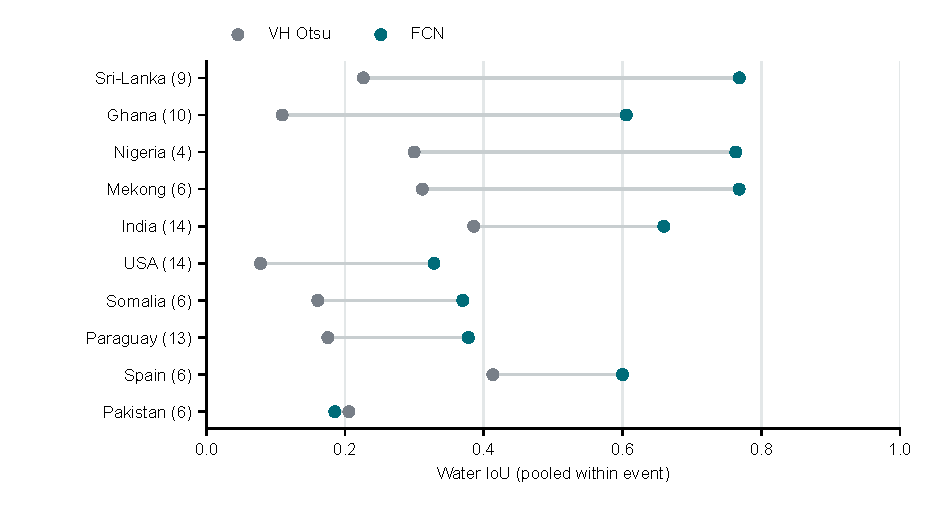
\includegraphics[width=.98\linewidth]{figures/event-iou.pdf}
\caption{官方测试清单内的事件分组。点按组内汇总混淆计数计算，括号为有共同有效像元的图块数。各组是配对描述，不是独立泛化试验或显著性检验。}
\label{fig:official-events}
\end{figure}

按组汇总后，巴基斯坦分组的 Otsu IoU 为 0.206，FCN 为 0.185（图~\ref{fig:official-events}）。该组只有六个图块；网络同时增加误报与漏检，因此不能用“更偏重召回”解释这次排序反转。图~\ref{fig:official-cases} 在两个方法 IoU 均定义的图块中，按 FCN 减 Otsu 的差值取一正一负两个极端。斯里兰卡案例中，阈值法在大块标注水面内部漏掉 176\,611 个像元，而 FCN 匹配了全部标注水体、同时多报 4\,704 个像元。巴拉圭案例中，网络追回了部分遗漏，河岸附近的误报却增至 29\,810 个像元，IoU 由 0.898 降到 0.624。图上能定位分歧集中在哪，但不能单凭回波断定河岸误报的地物成因。两幅极端图块不能代替逐事件统计。

\begin{figure}[H]
\centering
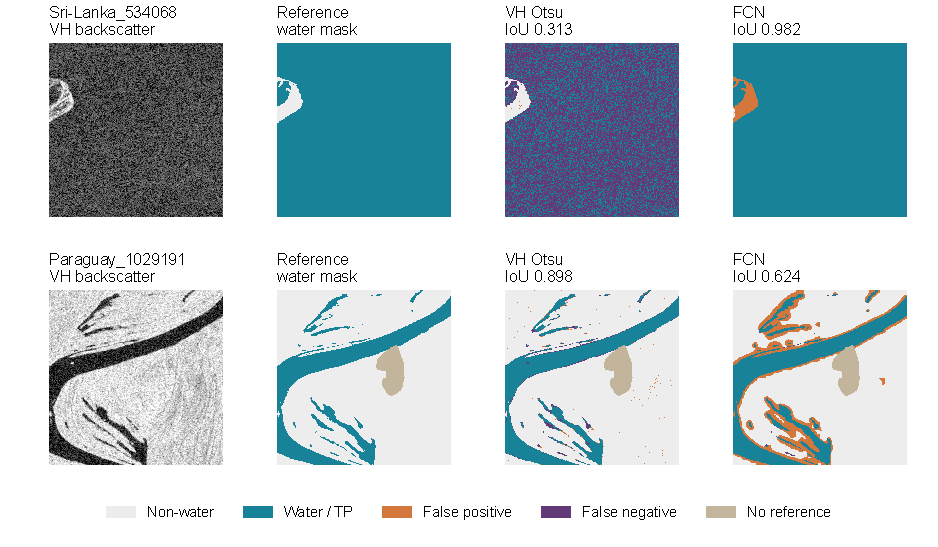
\includegraphics[width=.98\linewidth]{figures/cases.pdf}
\caption{FCN 减 VH Otsu 的图块 IoU 差值最大（上）及最小（下）的案例。VH 两行统一在 $[-32,-12]$ dB 显示；误差仅在共同有效区着色。}
\label{fig:official-cases}
\end{figure}

\subsection{事件级制图结果}
默认规则在 923.2944 \km 的共同覆盖域上产生 51.9024 \km 候选，约占研究区 5.62\%。候选高程中位数约为 $-0.67$ m，95 分位数约为 0.58 m，空间上主要集中在瓦伦西亚南部低地、农田和阿尔布费拉周边。这个空间形态与地形背景相容，但不能仅凭低海拔就把全部候选宣布为洪水。稳定暗水代理面积为 37.0704 \km，说明在灾后低散射区域中存在相当部分与稳定水体相关的像元，变化检测仍有必要保留“稳定水”和“新变化”的区分。

图~\ref{fig:candidate-map} 是候选专题图。青色为 SAR 变化候选，深蓝为稳定暗水代理，琥珀色实线为 EMS 参考边界，浅色虚线为分析范围。右侧列出观测日期与 20 m 网格。主图左、下图廓上的数字是 UTM 北坐标与东坐标，单位为米；指北针表示网格北。A3 原尺寸下，主图约为 $1:152\,000$、局部图约为 $1:103\,000$。主图上的黑框由 QGIS 链接到局部图，改变局部范围时框线随之更新\cite{qgis}。

\begin{figure}[H]
\centering
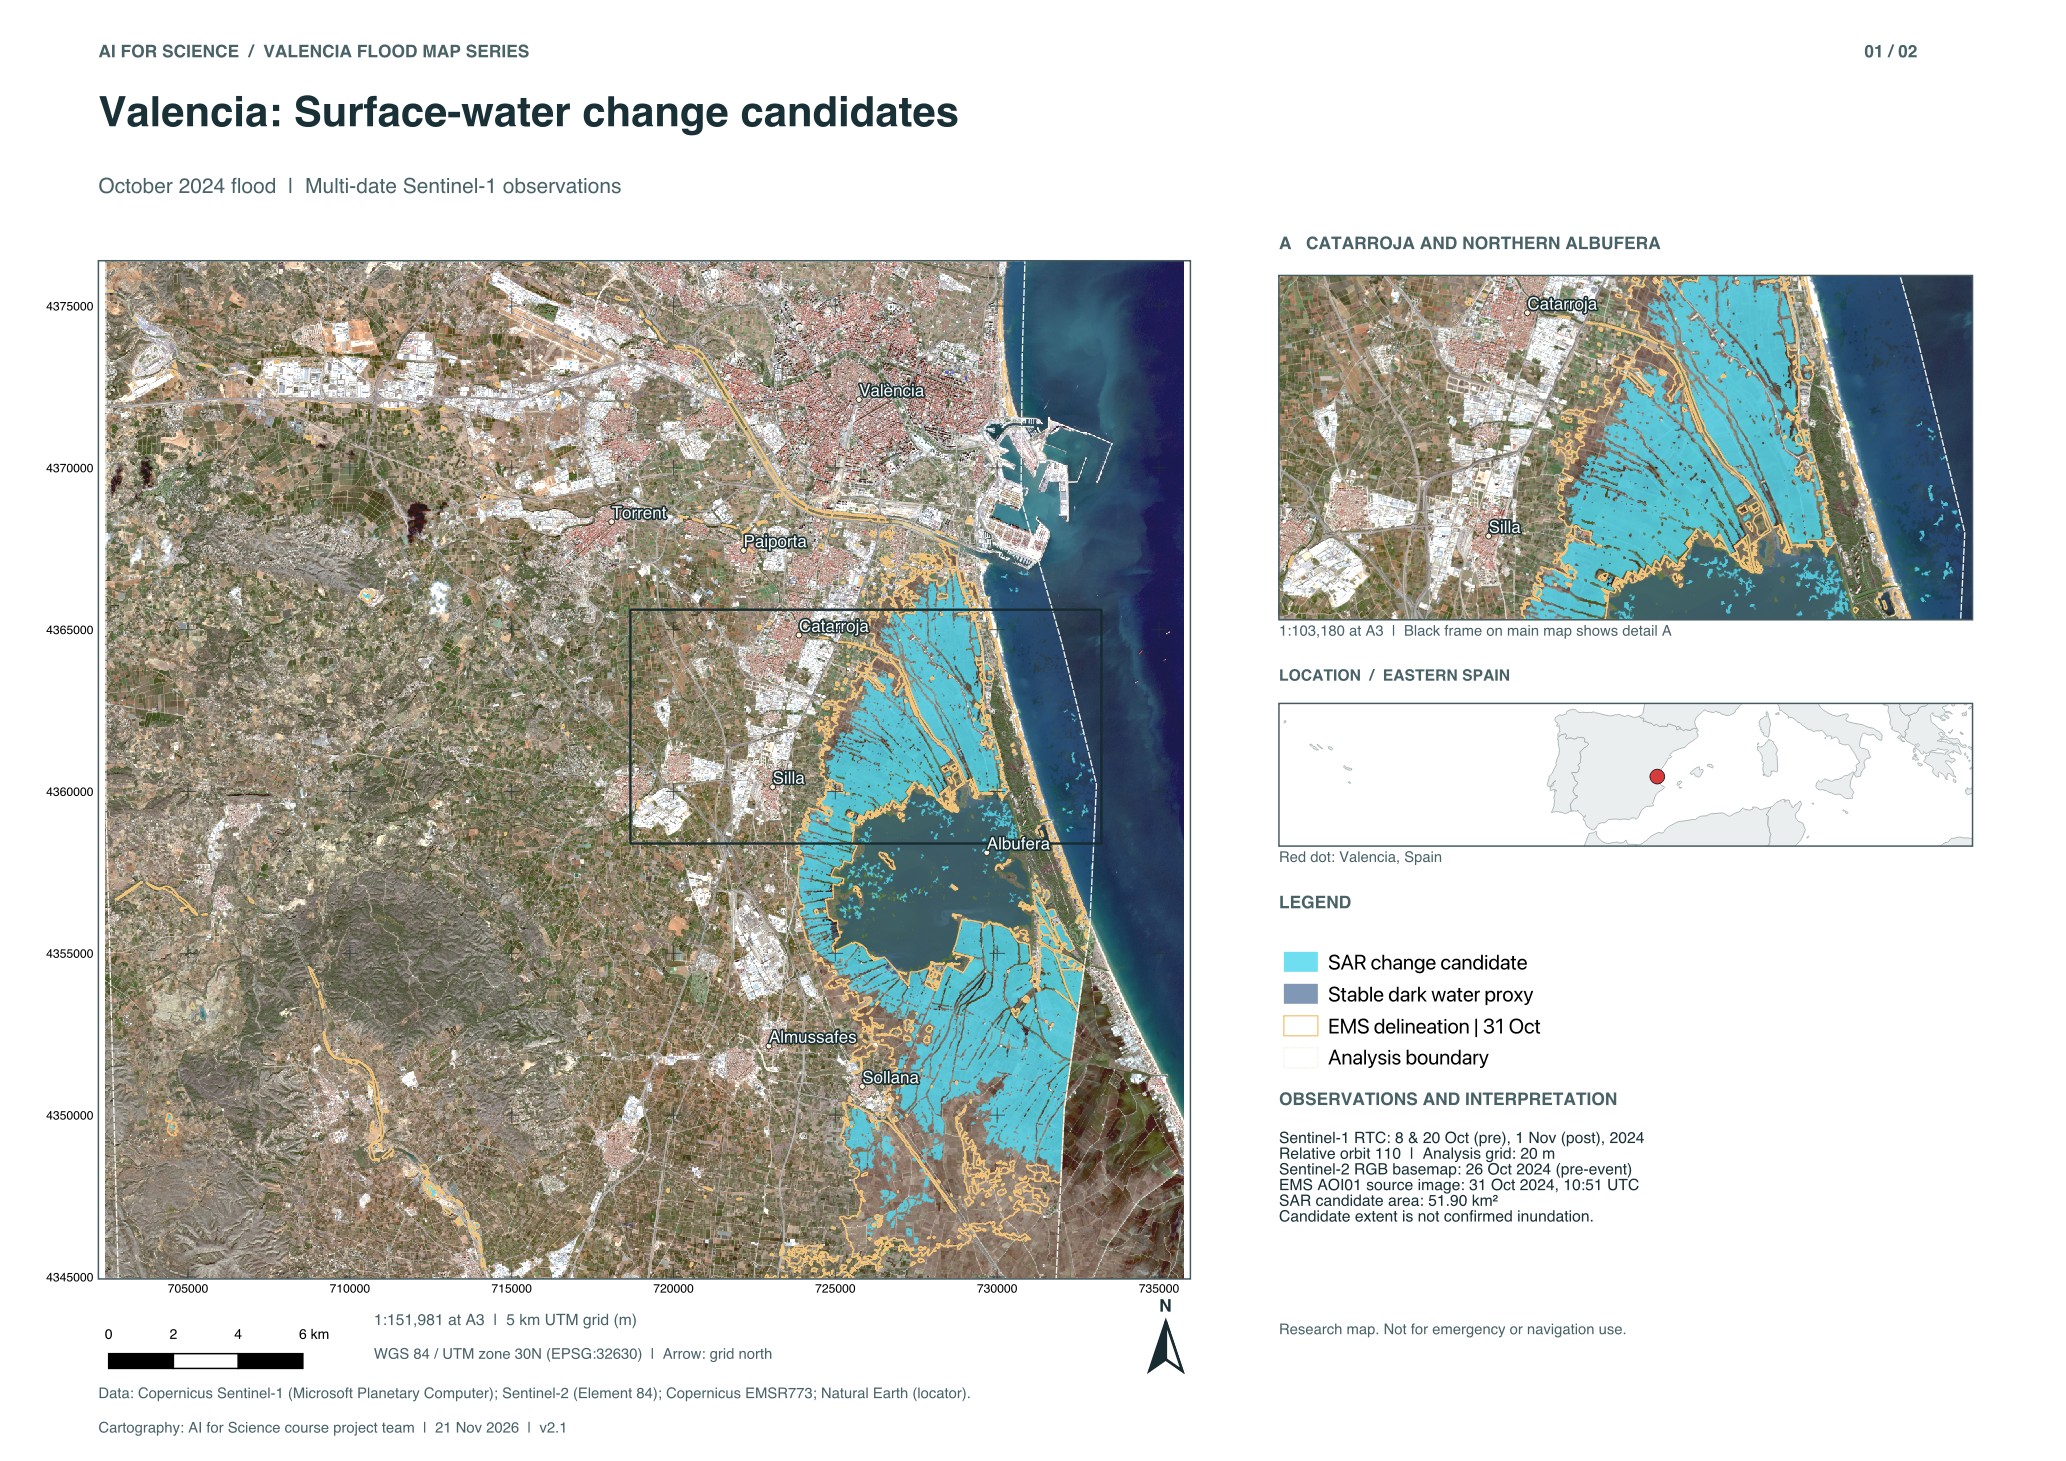
\includegraphics[width=.98\linewidth]{../event/maps/01-water-change.png}
\caption{瓦伦西亚事件的多时相 Sentinel-1 变化候选图。地图为 QGIS 可编辑布局的 PNG 导出，PDF 与 \code{Valencia-2024.qgz} 同时交付。}
\label{fig:candidate-map}
\end{figure}

\subsection{与异步 EMS 参考的比较}
EMS 参考在比较支持域内的面积为 93.5764 \km。候选图与其比较得到 $TP=126249$、$FP=3507$、$FN=107692$、$TN=2070788$，IoU 为 0.532，精确率为 0.973，召回率为 0.540，$F_1$ 为 0.694。高精确率说明候选图中的大部分像元也落在 EMS 参考范围内；较低召回率说明 SAR 候选只覆盖了参考范围的一部分。可能的原因包括观测日期差异、产品成图规则差异、湿地和农田的散射变化以及候选规则的保守性。由于参考并非同步真值，本文不把 FN 写成“算法漏检”，而写成“参考中未被 SAR 候选覆盖的区域”。

图~\ref{fig:agreement-map} 将空间关系直接制图。两源共同支持的区域集中在南部低地；仅 EMS 区域在局部呈紫色；仅 SAR 区域以橙色显示。这个图比单独给出 IoU 更适合做 Agent 的证据核验，因为用户可以看到“分歧在哪里”，而不是只接收一个不带空间含义的百分比。

\begin{figure}[H]
\centering
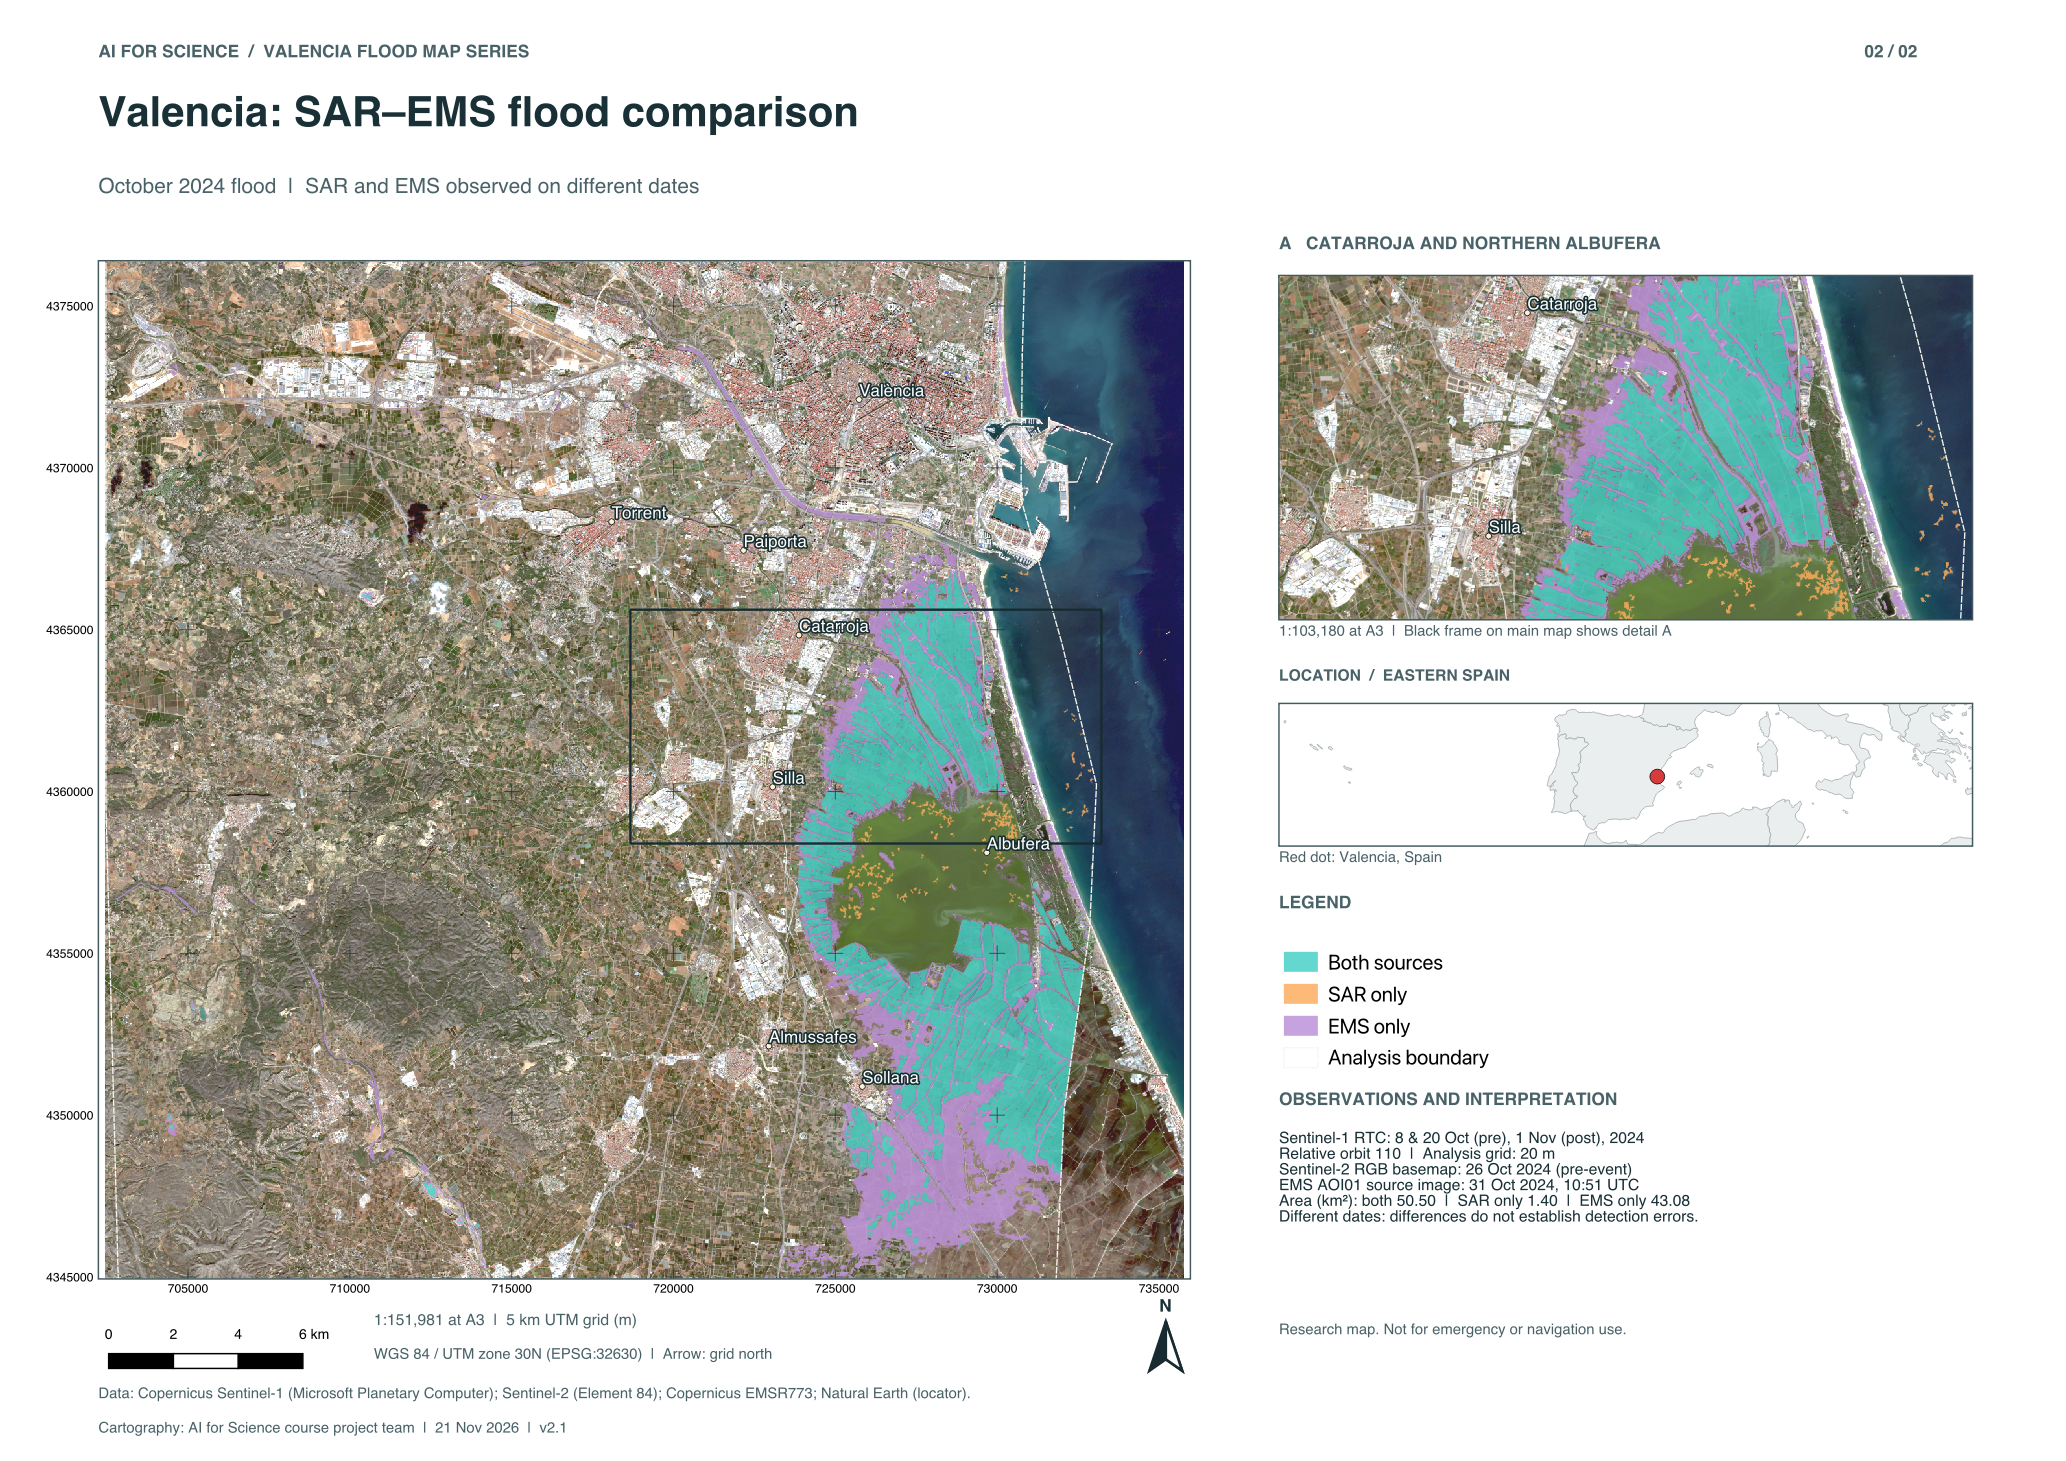
\includegraphics[width=.98\linewidth]{../event/maps/02-source-agreement.png}
\caption{SAR 变化候选与 Copernicus EMS 异步参考的一致/分歧图。图中分区不代表真值标签，而是两个制图来源的空间关系。}
\label{fig:agreement-map}
\end{figure}

\subsection{控制方法与变化检测的必要性}
灾后单期 Otsu 水体面积为 143.6408 \km，与 EMS 参考比较得到 IoU 0.411、精确率 0.481、召回率 0.739、$F_1$ 0.583。FCN 单期水体面积为 131.8676 \km，IoU 0.502、精确率 0.572、召回率 0.806、$F_1$ 0.669。FCN 在单期参考比较中优于 Otsu，但两者预测面积都明显大于变化候选 51.90 \km。这不是简单的模型优劣，而是任务定义不同：单期方法把永久水面和灾后积水放在同一个正类中；多时相方法尝试提取相对灾前的变化。

\begin{table}[H]
\centering
\caption{不同制图对象的结果对照。EMS 仅作为异步比较参考。}
\label{tab:methods}
\small
\begin{tabular}{lrrrrr}
\toprule
方法/对象 & 预测面积(\km) & IoU & 精确率 & 召回率 & $F_1$\\
\midrule
灾后 VH Otsu 单期水体 & 143.6408 & 0.411 & 0.481 & 0.739 & 0.583\\
灾后 FCN 单期水体 & 131.8676 & 0.502 & 0.572 & 0.806 & 0.669\\
多时相 SAR 变化候选 & 51.9024 & 0.532 & 0.973 & 0.540 & 0.694\\
VH Otsu 扣除稳定暗区 & 106.6852 & 0.525 & 0.646 & 0.737 & 0.688\\
FCN 扣除稳定暗区 & 96.4044 & 0.655 & 0.780 & 0.804 & 0.792\\
\bottomrule
\end{tabular}
\end{table}

扣除稳定暗区后，FCN 的 IoU 达到 0.655，高于多时相规则的 0.532；后者在三者中与 EMS 重叠的候选占比最高，但覆盖了较少参考区域。若任务更重视找全待复核区域，FCN 扣除稳定暗区是本事件值得保留的工具；若任务更重视筛出变化证据较强的区域，则多时相规则提供更保守的结果。两种判断均依赖同一个异步参照和单一研究事件，不能据此确定通用默认方法。

\subsection{安慰剂、参数与地形分层}
灾前安慰剂面积 16.6076 \km，约为默认候选的 32.0\%。这说明两次灾前观测之间仍会产生变化，但变化规则在事件前后产生了更强的响应。九组参数扫描的结果显示，严格共同支持区为 45.7604 \km，而宽松并集为 59.7580 \km。将默认候选面积简单写成一个精确值会掩盖参数不确定性，因此图和报告同时保留默认面积、安慰剂面积和稳定支持范围。

按高程分层，$<2$ m 区域候选与 EMS 的 IoU 为 0.608，精确率为 0.973，召回率为 0.618；2--10 m 区域 IoU 为 0.067，召回率为 0.067；$\geq10$ m 区域 IoU 为 0.061，召回率为 0.062。低地结果明显更好，符合洪涝影响在低洼区域更集中的直觉，但也提示高地的小面积积水、城市遮挡和参考产品稀疏会造成评价不稳定。这里的高程分层是解释性统计，不是把 DEM 当作水深。

\subsection{连续需求变更的真实执行}
产品先实跑两个连续任务，再通过浏览器真实表单提交第三个任务。第一轮统计全部已提供道路的 1 km 网格，第二轮改为 primary、primary\_link、secondary、secondary\_link 四类道路的 2 km 网格，第三轮进一步改为 residential 道路的 500 m 网格。三次操作分别留下 16、13、12 次工具调用和各一次截图读取。第二轮曾中断并恢复，因此其累计时间不用于与其他运行作速度比较；中断前后的实际响应都保留。

\begin{table}[H]
\centering
\caption{产品连续实例的独立数值核验。道路长度均为 AOI 内去重后的长度，暴露仅指与 EMS 轮廓平面重叠。}
\label{tab:product-runs}
\small
\begin{tabular}{lrrrr}
\toprule
道路条件 / 网格 & 格数 & 总长(m) & 暴露长(m) & 逐格核验\\
\midrule
全部 / 1 km &156&1\,298\,372.08&8\,027.37&通过\\
四类主干道 / 2 km &42&56\,848.18&443.52&通过\\
住宅道路 / 500 m &624&627\,080.26&277.59&通过\\
\bottomrule
\end{tabular}
\end{table}

三次结果不能按暴露长大小直接判断哪个区域更安全，因为道路集合和统计尺度不同。四类主干道路版本中，42 个格子有 20 个存在所选道路；住宅道路版本中，624 个格子有 286 个存在所选道路。其余格子的比例应为空，而不是零风险。四类主干道路的最高暴露率位于格号 38，约为 35.23\%；住宅道路的最高比例位于格号 551，约为 4.60\%。这些数字均来自工具表格和独立核验，不是语言模型估计。

第二轮完成后，第一轮地图仍能作为历史版本打开，但依赖追踪将其标记为不再满足当前分析参数。第三轮从已有历史创建新工作空间，保留前两轮的来源和结果。用户能够比较三份成果，而不是只能看到最后一段回答。这是产品层面可直接观察的 Agent 作用：新请求产生新的处理路径和实际数据文件，而非只改变文本解释。

\begin{figure}[H]
\centering
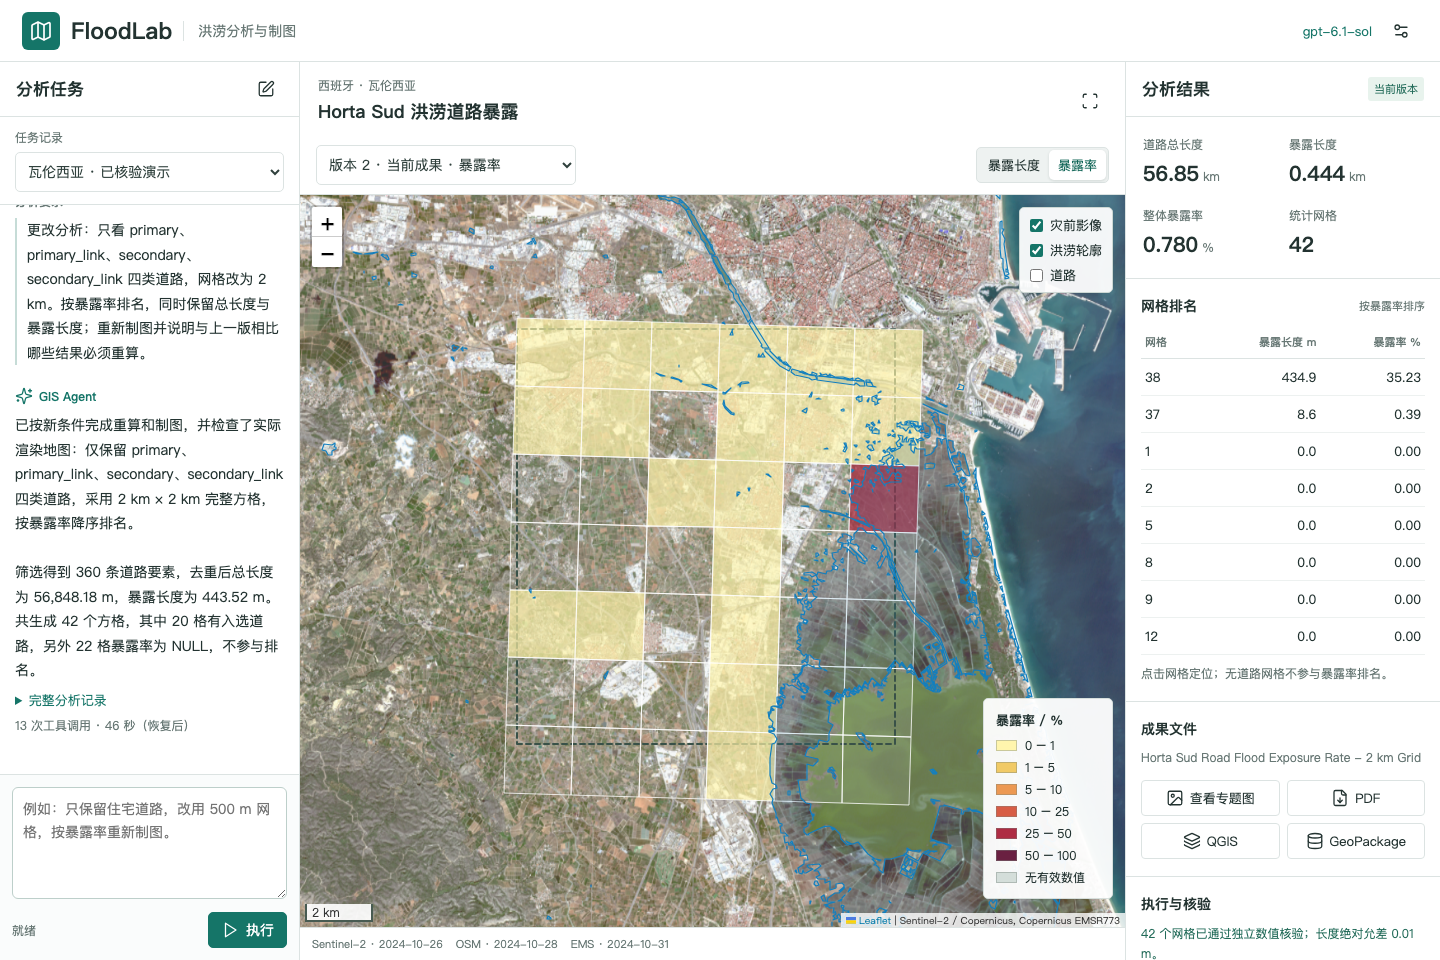
\includegraphics[width=\linewidth]{../workbench/qa/desktop.png}
\caption{瓦伦西亚实验期间的浏览器工作台（历史界面）。图中保留了当次运行的图层、排名与下载入口；0.6.0 桌面版已改为对话、地图与成果分视图。}
\label{fig:workbench}
\end{figure}

\begin{figure}[H]
\centering
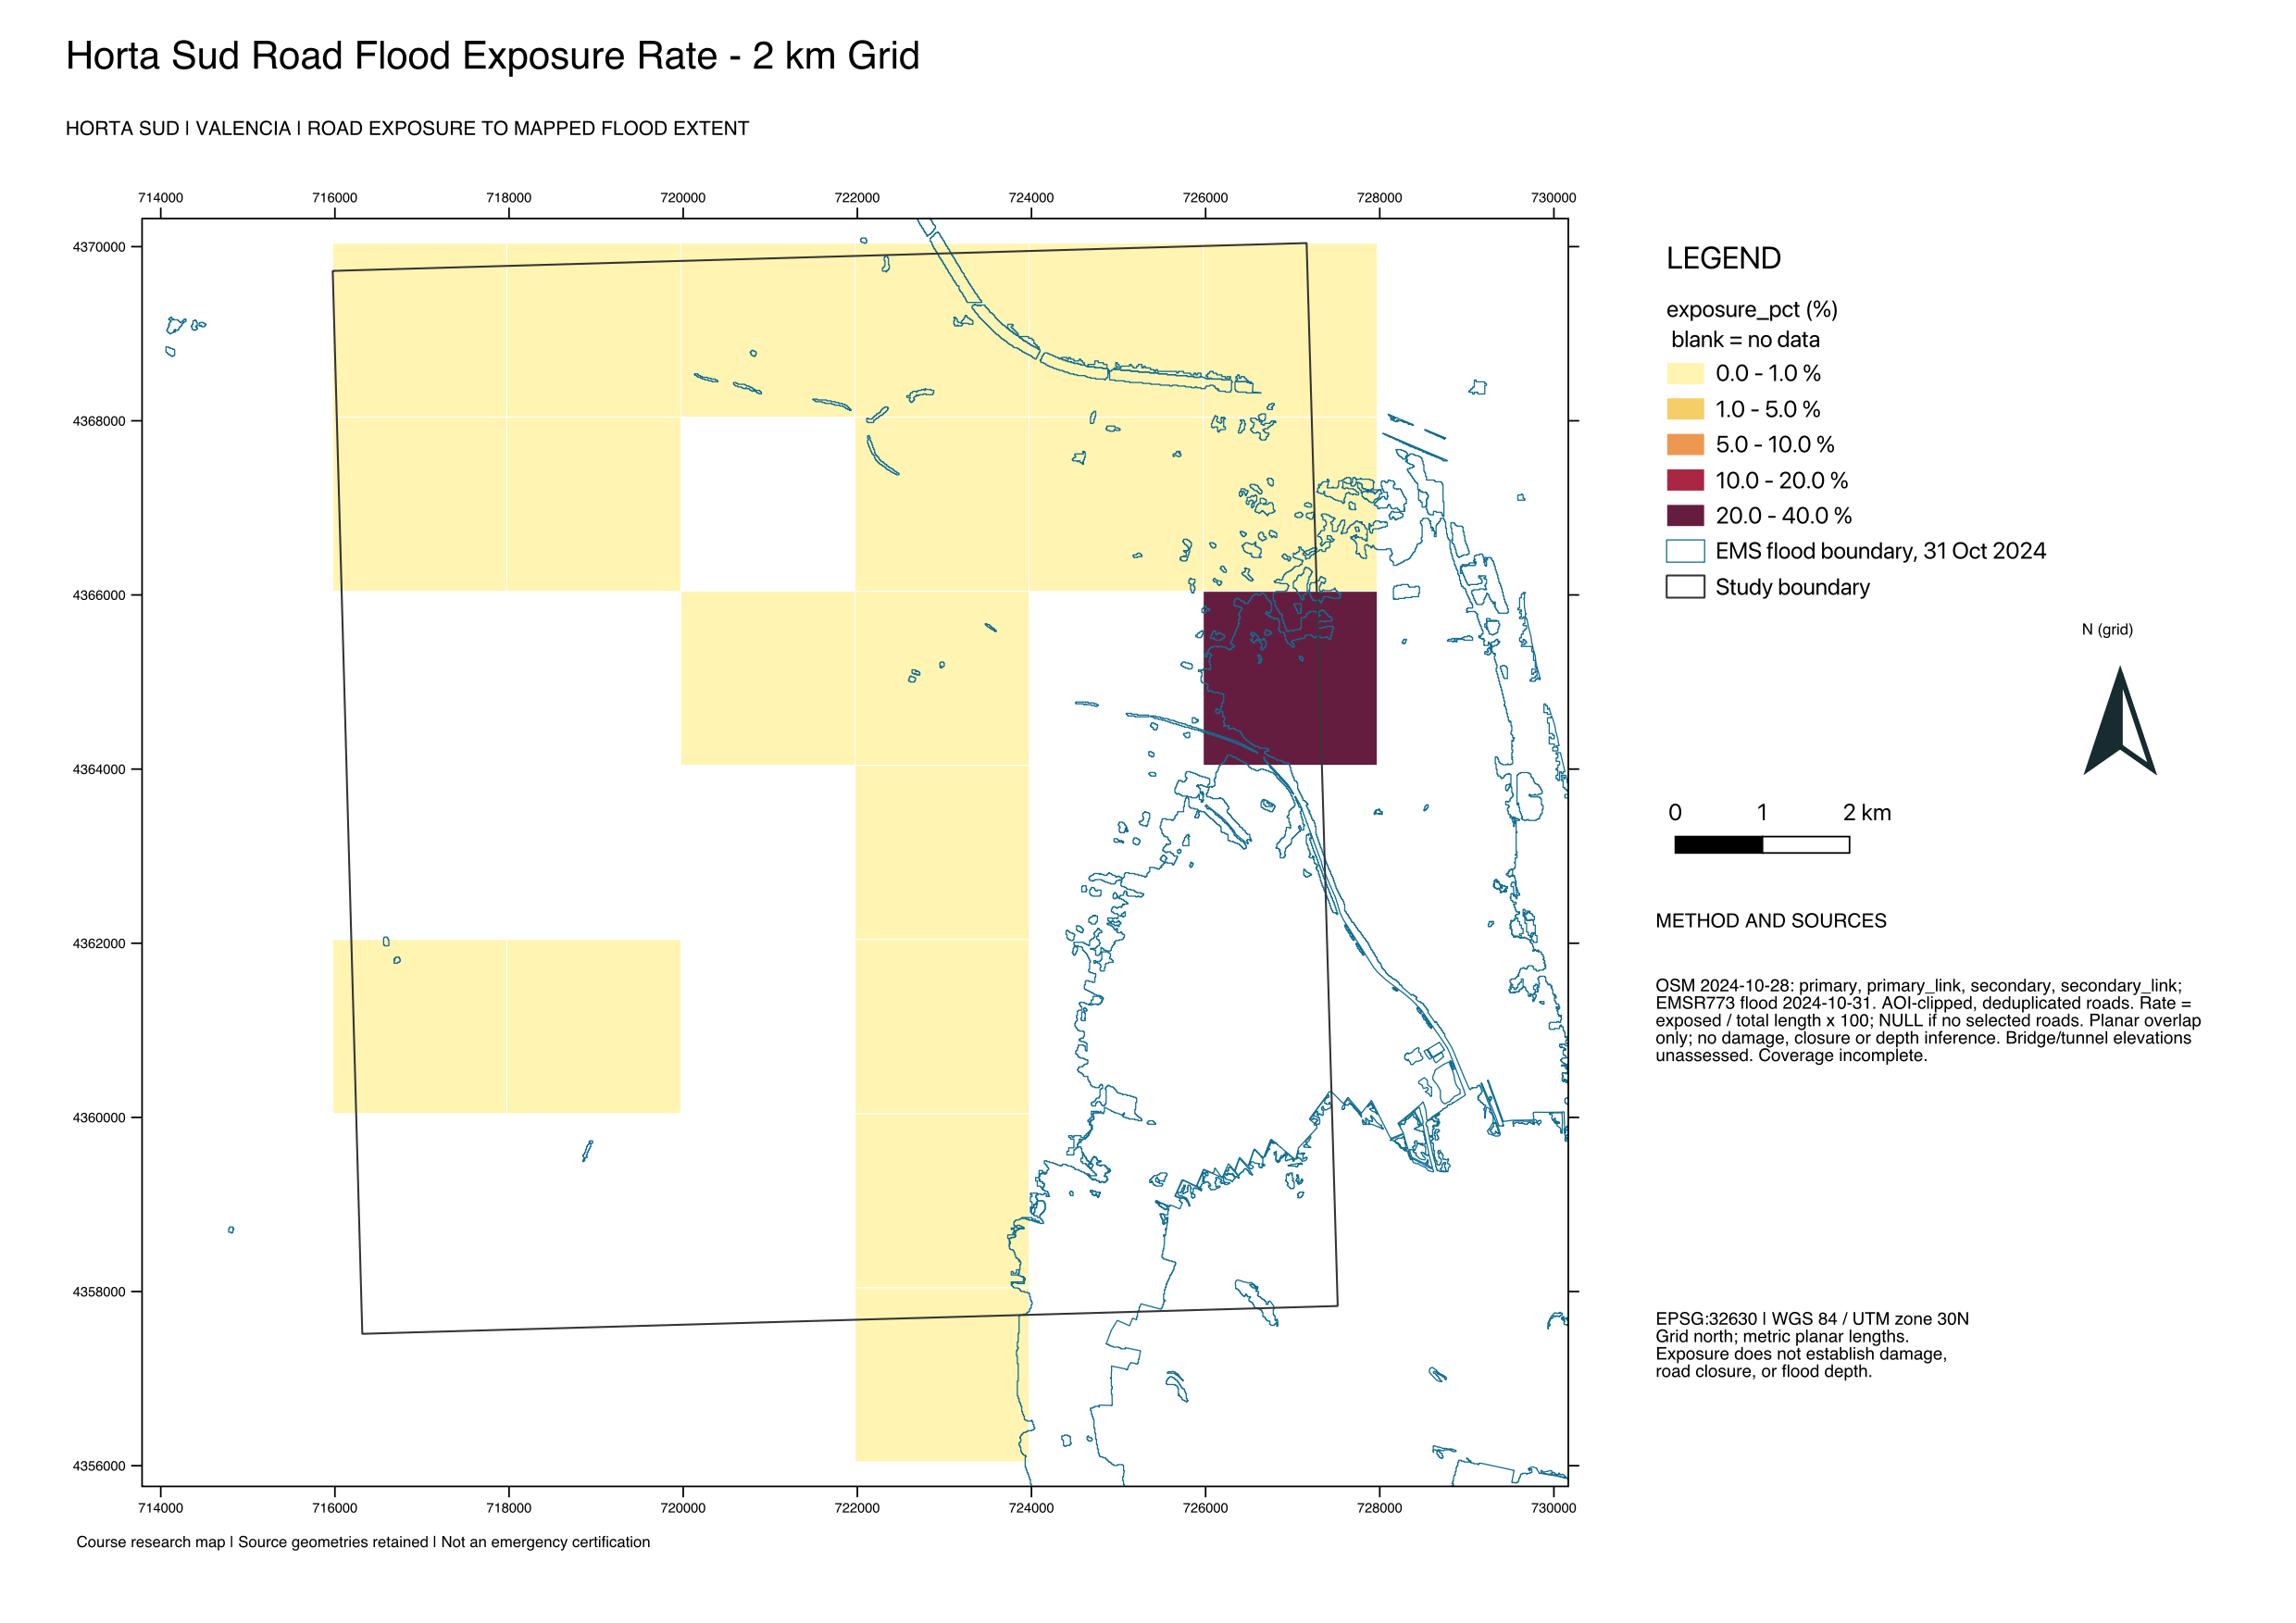
\includegraphics[width=\linewidth]{../event/runs/gis-agent-pilot-v2/horta_sud_major_roads_2km.png}
\caption{Agent 调用 QGIS 生成的四类主干道路 2 km 网格暴露率图。版面由确定性模板提供，分析图层、指标、分级和来源说明由实际调用指定；道路暴露不代表封路。}
\label{fig:agent-map}
\end{figure}

\subsection{非预装事件：克里特岛 Kastelli}
验收的第一问指定了希腊克里特岛、2026 年 10 月和 Kastelli，要求先查观测日期；第二问只说“那就分析这个区吧”，要求面积、1 km 网格排名和地图。因此，这验证了跨轮指代与非预装数据获取，不是让模型盲猜研究区。运行日志中先后出现事件检索、目录匹配、产品清单、下载和分析调用。EMS 激活编号为 EMSR933，产品编号为 2962，所选影像记录时间为 10 月 6 日 10:47。源图层标注包含积水范围和洪水痕迹，不能把两类面积之和称为这一时刻的全部明水面积。

QGIS 将 88 个多边形变换至等积坐标系 EPSG:6933，求几何并集后得到 0.241266 \km。与 1 km 网格相交后，20 格具有非零交叠。覆盖面积最大的格号为 8-11，对应 0.071973 \km，占该格面积的 7.20\%；该比例的分母是一个完整网格，不是全区观测面积。程序检查各格交叠面积之和与并集面积一致。这是同一输入上的面积守恒检查，不能代替瓦伦西亚实验中的独立程序复核，更不能证明原始产品没有漏绘。
\begin{figure}[htbp]\centering
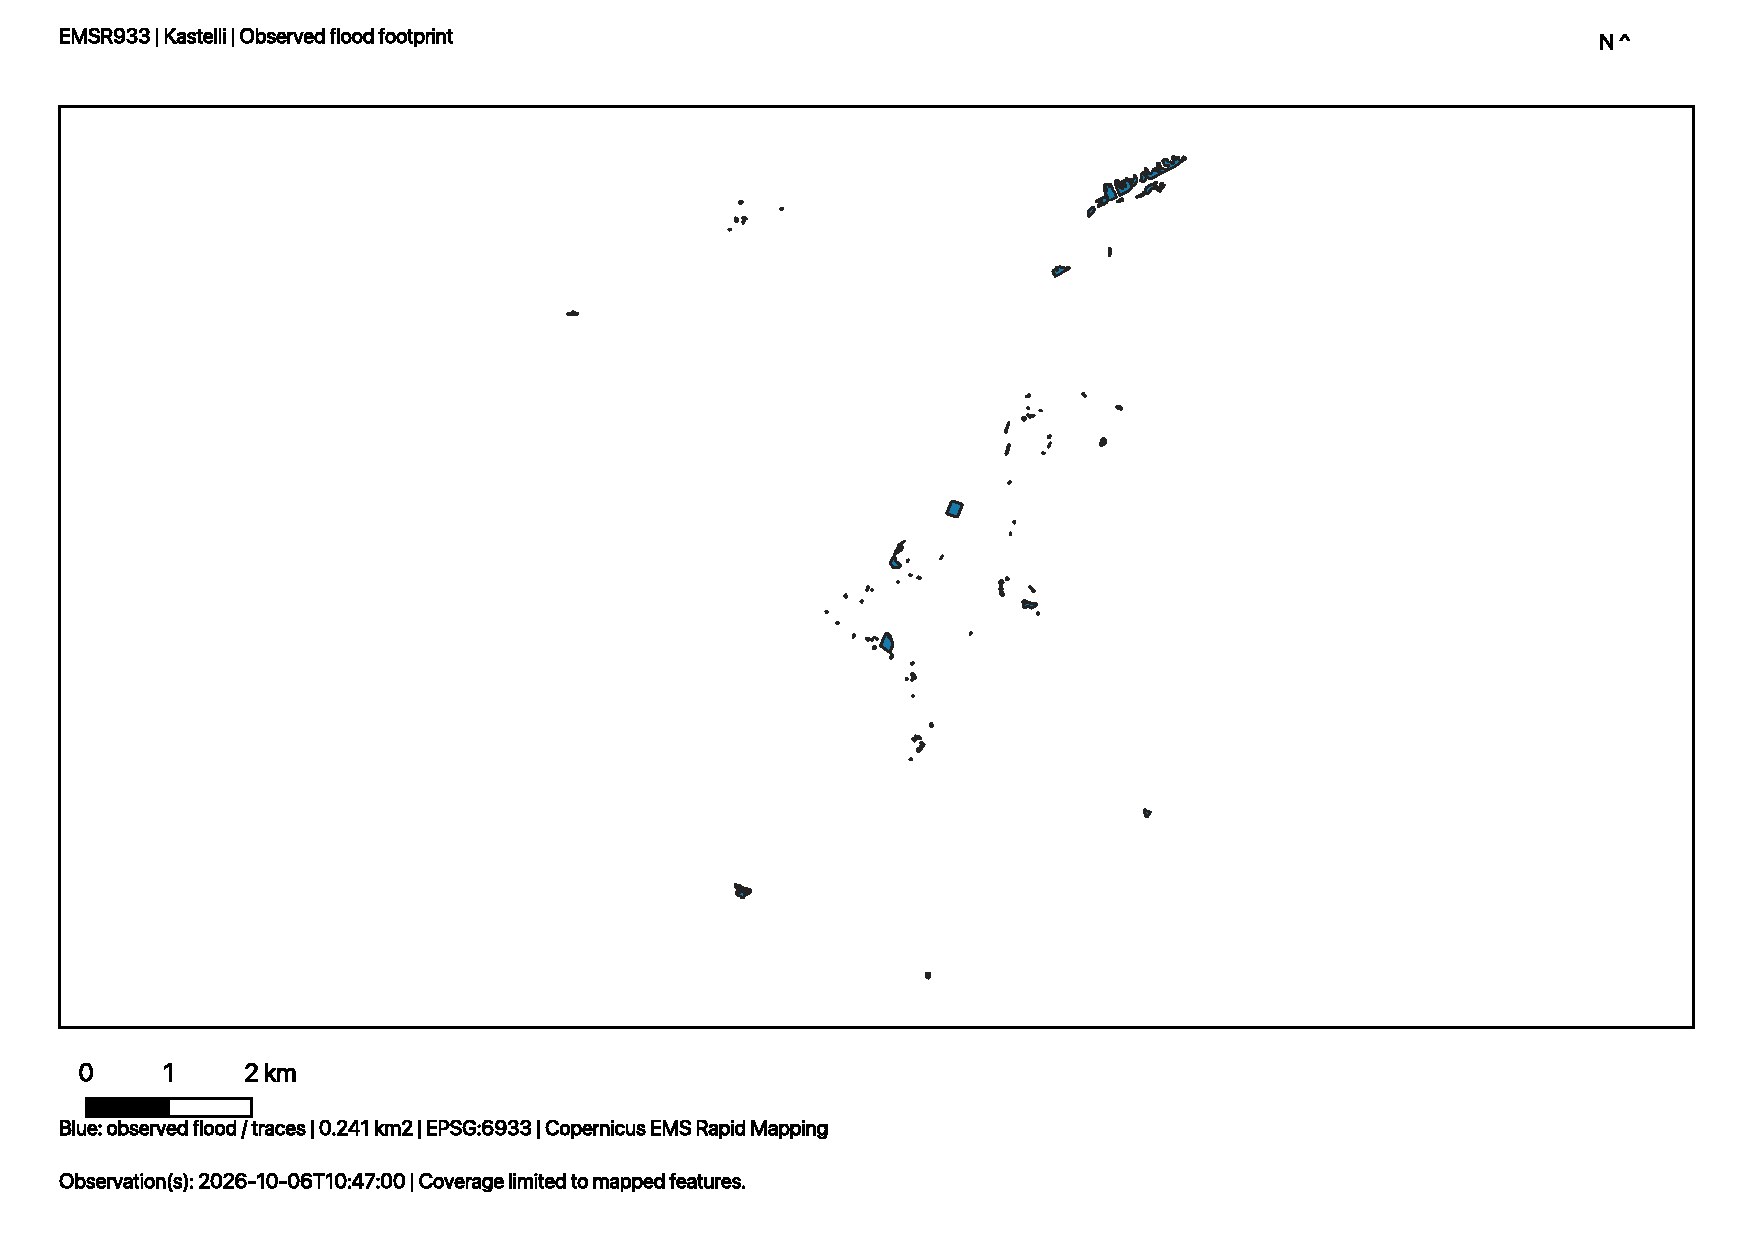
\includegraphics[width=.94\linewidth]{figures/kastelli-observed.pdf}
\caption{由非预装观测产品生成的 Kastelli 专题图。蓝色表示该产品制图的积水及洪水痕迹；空白处不等于经核实未受灾。}
\end{figure}

本次对话生成了专题图 PDF、网格 GeoJSON、统计 JSON 及可编辑 QGIS 工程。另起对话、再次选同一个父文件夹时，新对话获得不同子目录，且没有继承前一对话的成果。应用能按历史会话重新打开地图；这项测试验证文件归属与交付路径，不是灾害识别精度测试。

\subsection{对照实验与证据边界}
三种条件均完成四轮问题。前两轮的六个结果图层逐格通过独立核验，最大长度绝对差约为 $5.1\times10^{-11}$ m，低于预设容差；对应的地图均使用本轮计算图层和正确指标。完整模式用百分比表示暴露率，另外两组用 0--1 分数；核验先统一单位再比较，未把字段名称不同误判为计算错误。

\begin{table}[H]
\centering
\caption{探索性三条件对照。每条件仅一条四轮轨迹；“边界”指水深与封路两问，未做显著性检验。}
\label{tab:gis-comparison}
\small
\begin{tabular}{lrrrrr}
\toprule
条件 & 数值任务 & 边界回答 & 调用数 & 读图数 & 总时长(s)\\
\midrule
依赖追踪 + 图像 &2/2&2/2&27&2&194.7\\
通用工具 + 图像 &2/2&2/2&28&2&200.3\\
依赖追踪，无图像 &2/2&2/2&28&0&185.4\\
\bottomrule
\end{tabular}
\end{table}

上述结果没有显示依赖追踪或图像输入在这批任务上提高成功率。通用条件自行正确重算了新道路集合和新网格，未尝试复用失效结果；完整模式因此没有在自然轨迹中触发旧结果阻断。带图像的两组都调用了截图读取，但没有基于截图再次修改地图。无图像模式也导出了字段、单位与范围正确的地图，并主动说明未进行图面目视检查。不能因为实现了某项机制就认定该机制已经产生增益。

六张地图均有图例、比例尺、网格北、坐标和来源。这里按要素与指标核对地图，未做视觉质量排名。完整结果可在 \code{event/runs/gis-comparison/} 查看。

三组对最大水深均回答现有图层不足、应记为未知而非零；对实际封路长度也明确区分 443.52 m 的平面暴露与缺少通行观测的未知长度。两问没有新增工具调用，说明回答来自已经提供的数据说明和历史工具上下文，并非系统另行获取了水深或交通信息。此处通过只意味着没有超出当前证据，不证明模型能够在未提示限制的开放问题中始终正确拒答。

供应商响应报告的累计 token 用量依次为 512\,381、518\,282 和 456\,904，包含每步重复输入的上下文及缓存 token，不是互不重复的文本量，也不等同于账单费用。时长含接口等待与本地处理，只有单次观测，不能据十余秒差异主张某种模式稳定更快。所有调用均未返回工具错误；这也意味着本组自然任务没有覆盖复杂错误恢复，相关机制仅由单独的故障测试检查。


\subsection{工程验证与失败记录}
界面检查覆盖桌面、平板和手机布局、历史版本、指标切换、图层开关、排名网格定位、PDF 下载、新任务清空旧指标及真实任务提交。浏览器自动化生成了可查看的截图与逐项检查记录；这些记录只表示指定操作通过，不代表真实用户可用性评分。图层核验通过也不能替代版面检查，因此报告与地图另作渲染检查，并保留可编辑 QGIS 工程。

旧版本的失败仍有解释价值。在 14 条单期改写题中，原工具循环通过 6 条，后续单动作路由通过 13 条；B09 要求由一期影像计算新增水面，模型仍调用 FCN 输出了单期面积，故记为失败。事件路由的 12 条预设任务虽全部通过，但包含规则恢复和固定管线，不能用于证明多步空间规划。新版报告将这两组数据保留为迭代记录，未合并进当前 GIS Agent 的成绩。

本轮还记录供应商首次模型请求返回 HTTP 502 的情况，未把失败请求替换成虚构响应。早期地图冒烟测试曾出现坐标注记拥挤，随后调整图框和注记位置；冒烟测试使用确定性调用，只用于检查工具是否可用，不计作 Agent 成功案例。对故障、语义误判和视觉问题分别记账，可以避免只展示最后漂亮的一张图。

\section{总结与反思}
\subsection{完成了什么，以及 Agent 用在哪里}
本项目完成了一个能提出任务、执行空间分析、查看真实地图并下载成果的本地应用。遥感基准证明上游工具已实际运行：官方清单的 90 个图块产生两套 GeoTIFF，88 个图块用于评价。事件实验补充多时相变化、安慰剂、参数敏感性与异步来源比较。GIS Agent 则在明确的数据范围内完成道路筛选、度量、网格统计和地图输出，三轮不同要求的结果均可从原始图层重新核对。

Agent 的作用是根据自然语言请求组合工具并维护任务上下文，确定性程序的作用是计算几何、保存来源和执行约束，二者没有互相替代。去掉语言模型，固定分析仍可由脚本完成，但新要求需要人重新组织操作；去掉 GIS 工具，模型只能给出无法验证的解释。因此课程成果主要是可检查的应用与工作流，而非新分割算法或已被证明优于通用助手的自主系统。

\subsection{为什么地图和历史版本属于分析本身}
地图上的单位、时间与图例是结论的一部分。百分比字段若被标作米，或一张旧网格地图被冠以新标题，即使底层数值某处正确，交付仍然错误。历史版本把任务定义与输出对应起来，来源说明让读者知道本次选的是 EMS 轮廓还是 SAR 候选，图例则说明颜色表达长度还是比例。可编辑工程和数据文件使这种关系可以继续检查，避免只有静态截图而无法定位计算对象。

现有两张事件图包含主图、局部图、定位图及完整观测时间；Agent 动态输出的道路图使用简化 A3 专题模板，具有图廓、坐标标注、图例、网格北、比例尺、投影、来源及证据说明。二者布局并不相同，不能把前者的所有元素概括成每张动态图都具备。地图均为科研专题图，未经过正式测绘成果质量认证，也不用于应急封路决策。

\subsection{尚不能支持的结论}
第一，上游水体、变化候选和下游暴露是不同对象。FCN 在官方图块上优于阈值法，不保证在瓦伦西亚变化检测中最优；EMS 与 SAR 日期不一致，其重叠指标不等于同期精度；道路与多边形相交不等于道路被淹没、损坏或封闭。本项目没有水深观测，因此无法估算最大水深或总体积。

第二，依赖追踪只覆盖实际声明的参数与上游图层。模型仍可能选择错误的字段、漏记依赖、误读请求或给出错误文字；程序不可能通过一个状态标签保证所有科学语义正确。图像反馈也只提供检查机会，若模型没有识别版面问题，看过截图本身不构成质量保证。

第三，瓦伦西亚三条件对照均来自同一研究区，每个条件只运行一次。新增克里特岛案例验证了另一个事件上的产品获取与几何分析，但不是第二组对照，也不是对检索覆盖率的抽样评估。下一步应在预先指定的多个事件上记录匹配、下载、计算和交付各阶段的失败比例，并与获得同样工具和数据的通用 Agent 比较。

第四，公开数据与软件环境存在可移植性成本。OSM 覆盖和标签有局限，历史数据接口可能变动；QGIS、Python 和字体版本会影响重新运行和制图。归档原始响应、清单、散列、依赖锁和字体许可可以帮助复现，但模型 API 的返回不能保证逐字重现。报告把“可复算的几何结果”与“随机模型轨迹可重复执行”区分开，不要求二者具有相同含义。

\subsection{课程实践中的人工判断}
用户在讨论中明确指出原版仅做动作路由、不能体现 Agent 作用，并要求规范地图和可使用产品。这些实际判断推动了研究问题和底层实现的改变，是本项目已有的人工参与记录。代码编写、运行、核查和报告组织由 Codex 协助；当前没有收到具名成员对全部产物的独立签认。因此报告不填写虚构的个人实验贡献，也不把自动测试称为学生审核。成员最终应根据自己实际复跑、读图和修订的内容补充记录。

这次实践的重要认识是：产品演示、算法精度和科学证据是三个不同的评价对象。界面流畅不说明地图数值正确，数值一致不说明数据代表真实灾情，而日志完整也不说明学生理解了全过程。只有把每一项主张对应到可查看的输入、操作、输出及人工判断，课程成果才既能演示，也能接受追问。

\appendix
\section{团队分工与人工核对}
团队成员的研究背景分别覆盖遥感与视觉、机器人学习、多模态模型、具身智能与物理仿真。姓名据提供的名单填写；个人实际贡献、组长和培养单位未获最终确认。Codex 协助技术核查、代码、实验与文档；Qwen2.5-3B-Instruct 用于旧路由；新版 GIS Agent 实际调用用户授权的第三方模型接口。项目未调用磐石平台。重要操作和修改见 \code{EXPERIMENT_LOG.md}，独立学生审核仍待据实登记于 \code{TEAM_REVIEW.md}。

本报告依课程模板采用引言、任务设计与实施方法、结果与分析、总结与反思四章及附录。交付为用户要求的中文 LaTeX 与 PDF，中文字体采用随包附许可证的思源字体，以保证跨机器编译；不是原 Word 模板字体的精确复制。成员学号、培养单位和最终签认应由学生确认，不由模型推测。

\section{代码结构与复现命令}
\begin{itemize}
\item \code{event/acquire.py} 下载并记录 Sentinel-1、Sentinel-2、DEM 与 EMS 资料；
\item \code{event/analyze.py} 完成多时相变化、安慰剂、控制方法、指标、敏感性和地形分层；
\item \code{event/cartography.py} 在 QGIS 中生成两个 A3 布局、PDF、PNG 和 QGZ；
\item \code{event/publish_agent.py} 执行意图路由、证据门控、出版和 12 条基准任务；
\item \code{event/gis_agent.py} 执行新版真实模型与工具循环，\code{gis_tools.py} 提供 QGIS 原子操作；
\item \code{event/benchmark_gis.py} 冻结并执行三条件对照，\code{verify_gis.py} 独立核对逐格统计；
\item \code{workbench/server.py} 与 \code{workbench/public/} 提供本地产品；
\item \code{event/products/} 保存 GeoTIFF、GeoJSON、JSON 和 CSV；
\item \code{event/maps/} 保存最终地图和可编辑 QGIS 工程；
\item \code{event/runs/benchmark.json} 保存 Agent 的逐题轨迹、阻断理由和文件散列。
\end{itemize}

先按 README 安装锁定依赖、QGIS 与工作台依赖。核心命令如下：
\begin{verbatim}
uv run --no-sync python floodlab.py run --split test --device cpu
.venv/bin/python workbench/server.py --ask-key
.venv/bin/python event/benchmark_gis.py
.venv/bin/python -m pytest -q
latexmk -xelatex -cd -outdir=build report/main.tex
\end{verbatim}
上述命令用于研究源码环境；无需安装开发环境的用户可直接使用 0.6.0 桌面包，QGIS 已随包提供。检索留痕见 \code{desktop/qa/search-051.json}，跨事件下载、分格计算和工作区隔离的验收记录见 \code{desktop/qa/project-check.json}。冻结的瓦伦西亚对照保留其原始版本与模型轨迹，不追溯改写成 Pi 的实验结果。

\section{交付物与证据边界清单}
辅助工作中使用了研究方案、科研写作、文献核验、PDF 检查与本地站点开发相关 Skills；
它们用于组织代码、材料和检查流程，不是新的遥感模型，也不构成学生已完成操作的记录。
数据来源、许可与下载请求分别归档于输入清单和来源元数据。下表区分各类工件能支持的主张。\par
{\fontsize{11pt}{16pt}\selectfont
\begin{longtable}{p{62mm}p{80mm}}
\toprule
交付物 & 可以支持的结论\\
\midrule
\code{01-water-change.pdf/png} & 研究区内的多时相 SAR 变化候选及其地图位置\\
\code{02-source-agreement.pdf/png} & SAR 候选与 EMS 异步参考的空间重叠和分歧\\
\code{Valencia-2024.qgz} & 可在 QGIS 中再次打开、检查图层和布局的工程\\
\code{analysis.json} & 参数、面积、混淆计数、敏感性和高程分层统计\\
\code{benchmark.json} & 12 条 Agent 任务的动作、阻断理由和导出记录\\
\code{workbench/} & 本地交互产品及浏览器操作检查\\
\code{gis-agent-pilot-v2/} & 前两轮真实空间分析、地图和独立核验\\
\code{workbench_d0e0a1f802/} & 浏览器提交的第三轮分析及独立核验\\
\code{gis-comparison/} & 三条件冻结协议、原始模型返回及评价\\
\code{report/build/main.pdf} & 对数据、方法、结果和局限的完整说明\\
\bottomrule
\end{longtable}
}

\clearpage
{\fontsize{11pt}{16pt}\selectfont
\begin{thebibliography}{99}
\bibitem{sen1}
Bonafilia D, Tellman B, Anderson T, Issenberg E.
Sen1Floods11: A georeferenced dataset to train and test deep learning flood algorithms for Sentinel-1.
IEEE/CVF Conference on Computer Vision and Pattern Recognition Workshops, 2020.
\bibitem{senrepo}
Cloud to Street. Sen1Floods11 v1.1: test split, checkpoint storage and inference notebook.
\url{https://github.com/cloudtostreet/Sen1Floods11}.
\bibitem{planetary}
Microsoft Planetary Computer. Sentinel-1 RTC STAC collection and cloud access documentation.
\url{https://planetarycomputer.microsoft.com/}.
\bibitem{ems}
Copernicus Emergency Management Service. EMSR773 Valencia activation and rapid mapping products.
\url{https://mapping.emergency.copernicus.eu/}.
\bibitem{otsu}
Otsu N. A threshold selection method from gray-level histograms.
IEEE Transactions on Systems, Man, and Cybernetics, 1979, 9(1): 62--66.
\href{https://doi.org/10.1109/TSMC.1979.4310076}{doi:10.1109/TSMC.1979.4310076}.
\bibitem{qgis}
QGIS Development Team. QGIS User Guide and PyQGIS Developer Cookbook.
\url{https://docs.qgis.org/}.
\bibitem{qwen}
Qwen Team. Qwen2.5 technical report. arXiv:2412.15115, 2024.
\bibitem{giscopilot}
Akinboyewa T, Li Z, Ning H, Lessani M N.
GIS Copilot: Towards an Autonomous GIS Agent for Spatial Analysis.
arXiv:2411.03205v4, 2024.
\url{https://arxiv.org/abs/2411.03205v4}.
\bibitem{cartoagent}
Wang C, Kang Y, Gong Z, et al.
CartoAgent: a multimodal large language model-powered multi-agent cartographic framework for map style transfer and evaluation.
arXiv:2505.09936v1, 2025.
\url{https://arxiv.org/abs/2505.09936v1}.
\bibitem{osm}
OpenStreetMap contributors. OpenStreetMap historical road data; Open Database License.
\url{https://www.openstreetmap.org/copyright}.
\end{thebibliography}
}

\end{document}
